\chapter{User guided synthesis}
\label{ch:userguided}

This chapter presents the Termite device driver synthesis toolkit which builds on the game formalism of Chapter~\ref{ch:game_formalism} to create a practical driver synthesis tool.

One for the main challenges of driver synthesis is to enable developers to create drivers through a well-defined, predictable sequence of steps. In this chapter, I address this challenge through three key design objectives:
\begin{itemize}
    \item Ease of developing specifications for driver synthesis.
    \item Ease of debugging synthesis errors due to incorrect specifications.
    \item Enabling the benefits of automation without sacrificing the flexibility of conventional driver development.  
\end{itemize}
    
Termite addresses the first objective through a high-level specification language whose syntax and semantics are close to those of familiar imperative programming languages like C.  In addition, it facilitates the development of modular specifications and thus enables a high degree of specification reuse. Termite addresses the second objective by developing powerful debugging techniques that help the developer identify and fix specification defects through a well-defined process, similar to how conventional debuggers help troubleshoot implementation errors.  Finally, Termite's methodology strikes the balance between automation and flexibility by generating driver code in a user guided fashion, where the user can interactively alter or amend automatically generated code, while the synthesis tool verifies user changes on the fly.

\section{Introduction}\label{sec:user_guided_intro}

\subsection{Overview of \termite} Figure~\ref{f:termite} gives an overview of the driver synthesis process, described in detail in the rest of this chapter.  \termite takes four specifications as its inputs: 

\begin{enumerate}
    \item a device model that simulates software-visible device behaviour, 
    \item an OS model that specifies the requests to the driver that the OS may make and how the driver must respond,
    \item a driver template that contains driver entry point declarations and, optionally, their partial implementation to be completed by \termite,
    \item and, a device class specification that declares the interfaces that the operating system and device supply for a specific class of devices.
\end{enumerate}

\noindent Items (1) and (2) are the device and operating system specifications of Section~\ref{sec:composition}. Items (3) and (4) are auxiliary specifications to assist in driver code generation and specification reuse.

\begin{figure}
    \center
    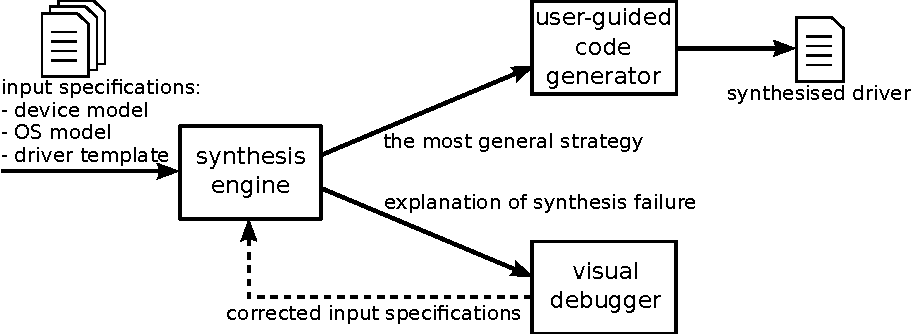
\includegraphics[width=\linewidth]{imgs/termite.pdf}
    \caption{\termite synthesis workflow.}\label{f:termite}
\end{figure}

Given these specifications, driver synthesis proceeds in two steps.  The first step is carried out fully automatically by the \termite game-based synthesis engine, which computes \emph{the most general strategy} for the driver---a relation $strat \subseteq S \times L$ (\ref{sec:intro_formal}) that represents all possible correct driver implementations.  This step encapsulates the computationally expensive part of synthesis.  At the second step, the most general strategy is used by the \termite code generator to construct one specific driver implementation in C with the help of interactive input from the user.

The synthesis engine may establish that, due to a defect in one of the input specifications, there does not exist a specification-compliant driver implementation.  In this case, it produces an explanation of the failure, which can be analysed with the help of the \termite debugger tool in order identify and correct the defect.

%        order to help the developer identify and correct the 
%        defect, the synthesis engine generates a data structure, 
%        called \emph{counterexample strategy}, representing device 
%        and OS behaviour that exposes the defect.  The driver 
%        developer uses the \termite visual debugger tool 
%        (Section~\ref{}) to explore the counterexample strategy, 
%        identify and correct the defect.  
        
%    \item We present the design an implementation of \termite in 
%    a top-down fashion.  We first explore the tool from the 
%    user's perspective.  
%
%        how input specifications for driver synthesis are created
%        
%        next, we explain how the user interacts with the \termite 
%        code generator to produce a well structured driver 
%        implementation.
%        
%        Next we look under the hood

\section{Specifications}
\label{s:specifications}

\hrule
\vspace{10pt}
\begin{center}
The design and implementation of the TSL specification language used in this section was performed by Dr. Leonid Ryzhyk. 
\end{center}
\hrule
\vspace{20pt}

Input to \termite consists of the four specifications, which model the complete system consisting of the driver, the device, and the OS as well as defining the interface between them, shown in Figure~\ref{f:actions}.  The OS and device models simulate the execution environment of the driver and specify constraints on correct driver behaviour.  The device model simulates software-visible device behaviour.  The OS model serves as a workload generator that issues I/O requests to the driver and accepts request completions in a way consistent with real OS behaviour.

\begin{figure}
    \center
    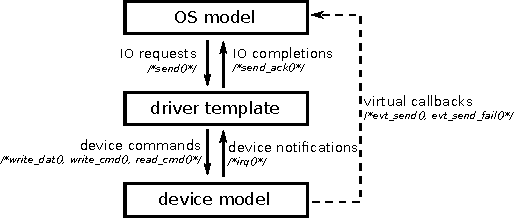
\includegraphics[width=0.85\linewidth]{imgs/actions.pdf}
    \caption{Input specifications for driver synthesis.  
    Labels in italics show interfaces from the running example
(Figure~\ref{f:ex_dev} and Figure~\ref{f:ex_os}).}\label{f:actions}
\end{figure}

The virtual interface between the device and the OS, shown with the dashed arrow in Figure~\ref{f:actions}, is used by the device model to notify the OS model about important hardware events, such as completion of I/O transactions and error conditions.  Methods of the virtual interface do not represent real runtime interactions between the device and the OS, but are used by the OS model to specify correctness constraints for the driver (see Section~\ref{s:virt}).

Finally, the driver template contains a partial driver implementation to be completed by \termite.  A minimal template consists of a list of driver entrypoints without implementation.  At the other extreme, it can provide a complete implementation, in which case \termite acts as a static verifier for the driver. By this I mean that it checks that the interactions between the driver software and the hardware ensure that all operating system requests are eventually fulfilled. Specifically, it ensures that the implementation satisfies the GR(1) objective (Section~\ref{sec:games_gr1}) expressed in the specification. It does not, for example, check for the absence of null pointer dereferences and similar defects that can be found by tools such as SLAM \cite{Ball_BKL_10}. In fact, \tsl is designed to express state machines, not arbitrary programs and complex data structures, and such defects are not expressible. Of course, this also limits the drivers that can be expressed.

All specifications are written using the \termite Specification Language (\tsl).  In line with the goal of making synthesis as close to the conventional driver development workflow as possible, \tsl is designed as a dialect of C with additional constructs for use in synthesis.  The full specification of the \tsl language is given in Appendix~\ref{ch:tsl_ref}. I introduce relevant features of \tsl throughout this section.

\termite allows the use of existing device specifications developed by hardware designers in driver synthesis as discussed in Section~\ref{sec:device_model}. This minimises the amount of work needed to develop specifications for every synthesised driver by maximising the reuse of specifications.  

Furthermore, the OS specification for the driver can be derived from a generic specification for a class of similar devices (e.g., network or storage).  Thus it is expected that additional per-driver effort will consist of: 
\begin{enumerate}
    \item inserting device-class callbacks (the TSL way of emitting device class events) in appropriate locations of the device model and 
    \item extending the OS specification to support device-specific features missing in the  generic OS specification.
\end{enumerate}

\subsection{Device model}
\label{sec:device_model}

The device model simulates the device operation at a level of detail sufficient to synthesise a correct driver for it.  To this end, it must accurately model external device behaviour visible to software.  At the same time, it is not required to precisely capture internal device operation and timing, as these aspects are opaque to the driver.

Such device models are routinely developed by hardware designers for the purposes of design exploration, simulation, and testing. They are widely used by hardware manufacturers in-house~\cite{cofluent} and are available commercially from major silicon IP vendors~\cite{vp}.  These models are known as \emph{transaction-level models} (TLMs) (in contrast to the detailed register-transfer-level models used in gate-level synthesis)~\cite{Cai_Gajski_03}.  A TLM focuses on software-visible events, or \emph{transactions}, such as a write to a device register or a network packet transmission.

Existing TLMs created by hardware designers can be used with minor modifications (explained in Section~\ref{s:virt}) for driver synthesis.  Model reuse dramatically reduces the effort involved in synthesising a driver and is therefore crucial to practical success of driver synthesis.  By reusing an existing model, Termite allows reuse of the effort invested by hardware designers in testing and debugging the model throughout the hardware design cycle, thus making driver synthesis less susceptible to specification bugs.  Finally, since TLMs are created early in the hardware design cycle, TLM-based driver synthesis can be carried out early as well, thus removing driver development from the critical path to product delivery.

Unfortunately, few TLMs are publicly available at the moment, which means that driver synthesis must be performed by  device vendors in-house.  However this is likely to change in the future.  A TLM does not expose internal implementation details of the device and is therefore not part of sensitive IP\@.  At the same time, there exist strong incentives for manufacturers to make device TLMs available to third-party vendors to test their software and hardware products for compatibility with the given device.

TLMs are written in high-level hardware description languages like SystemC and DML\@.  In order to use these models in driver synthesis, they need to be converted to \tsl.  This translation can be performed automatically, and the Termite team is currently working on a DML-to-\tsl compiler. This work is not yet complete and is not a contribution of this thesis. Therefore device models used in the experimental section of this paper are either manually translated from existing TLMs or written from scratch using TLM modelling style guidelines~\cite{dml_ug}.

\subsubsection{Running example}

\begin{figure}
\begin{tsllisting}[name=ex]
/* Device model */
template dev 

    /* Device internal state */
    uint8 reg_dat, reg_cmd, reg_status = 0; (*@\label{f:ex_dev:l:reg_decls}@*)

    /* device commands */
    controllable void write_dat(uint8 v) { (*@\label{f:ex_dev:l:start_access}@*)
        reg_dat = v; 
    };

    controllable void write_cmd(uint8 v) { 
        reg_cmd = v; 
    };

    controllable uint8 read_cmd() { 
        return reg_cmd; 
    };

    controllable uint8 read_status() { 
        return reg_status; 
    }; (*@\label{f:ex_dev:l:end_access}@*)

    /* internal behaviour */
    process ptx { (*@\label{f:ex_dev:l:start_xmit}@*)
        forever {
            wait (reg_cmd == 1); (*@\label{f:ex_dev:l:wait}@*)
            choice {(*@\label{f:ex_dev:l:atomic_start}@*)
                { 
                    os.evt_send(reg_dat); (*@\label{f:ex_dev:l:cb_succ}@*)
                    reg_status=0; 
                };
                { 
                    os.evt_send_fail(reg_dat);(*@\label{f:ex_dev:l:cb_fail}@*)
                    reg_status=1; 
                };
            };
            reg_cmd = 0; (*@\label{f:ex_dev:l:atomic_end}@*)
            /*drv.irq(); (see Section 4)*/(*@\label{f:ex_dev:l:irq}@*)
        };
    }; (*@\label{f:ex_dev:l:end_xmit}@*)
endtemplate
\end{tsllisting}
\caption{Trivial serial controller device specifications.}
\label{f:ex_dev}
\end{figure}

Figure~\ref{f:ex_dev} shows a fragment of a model of a trivial serial controller device used as a running example.  The fragment specifies the send logic of the controller, which allows software to send data characters over the serial line.  The model is implemented as a \tsl \emph{template}, TSL's mechanism for managing namespaces (Section~\ref{s:o:templates}).  The template encapsulates data and code that manipulates the data, similar to a class in OOP.

The software interface of the device consists of data, command, and status registers declared in line~\ref{f:ex_dev:l:reg_decls}.  The registers can be accessed from software via the \src{write\_dat}, \src{write\_cmd}, \src{read\_cmd}, and \src{read\_status} methods (lines~\ref{f:ex_dev:l:start_access}--\ref{f:ex_dev:l:end_access}).  The \src{controllable} qualifier denotes a method that is available to the driver and can be invoked from synthesised code.

The transmitter logic is modelled in lines~\ref{f:ex_dev:l:start_xmit}--\ref{f:ex_dev:l:end_xmit}.  It is implemented as a \tsl \emph{process}.  A \tsl specification can contain multiple processes.  The choice of the process to run is made non-deterministically by the scheduler.  The process executes atomically until reaching a \src{wait} statement or a controllable placeholder (see below).

In line~\ref{f:ex_dev:l:wait}, the transmitter waits for a command, issued by the driver by writing value $1$ to the command register.  Upon receiving the command, it sends the value in the data register over the serial line.  The transmission may fail, e.g., due to a serial link problem.  The device signals transmission status to software by setting the status register to $0$ or $1$.  Finally, it clears the command register, thus notifying the driver the request has completed.

Internally, the transmitter circuit consists of a shift register and a baud rate generator used to output data on the serial line.  These details are not visible to software and are abstracted away in the model.  The non-deterministic \src{choice} construct is used to choose between successful transmission and failure, without modelling the details of serial link operation.  Successful and failed transmissions are modelled using\src{evt\_send} and \src{evt\_send\_fail} events, explained in Section~\ref{s:os}.

\subsection{OS model}\label{s:os}

The OS model specifies the API mandated by the OS for all drivers of the given type.  For example, any Ethernet driver must implement the interface for sending and receiving Ethernet packets.  A separate specification is needed for each supported OS, as different OSs define different interfaces for device drivers.

Additionally, each particular device can support non-standard features, e.g., device-specific configuration options or transfer modes.  These features must be added as extensions to the generic OS specification in order to synthesise support for them in the driver.  \tsl supports such extensions in a systematic way via the template inheritance mechanism.  This is described in Appendix~\ref{ch:tsl_ref}.

\subsubsection{Running example}

\begin{figure}
\lstset{firstnumber=last}
\begin{tsllisting}[name=ex]
/* OS model */
template os 

    uint8 dat;
    bool inprogress, acked, success; (*@\label{f:ex_os:l:vars}@*)

    /* driver workload generator */
    process psend {
        forever {
            dat = *; /*randomise dat*/ (*@\label{f:ex_os:l:nondet}@*)
            inprogress = true;
            acked = false;
            drv.send(dat);
            wait(acked); (*@\label{f:ex_os:l:wait}@*)
        };
    };

    /* I/O completions */
    controllable void send_ack(bool status) { (*@\label{f:ex_os:l:ack}@*)
        assert (!inprogress && !acked && status == success);
        acked = true;
    };

    /* virtual callbacks */
    void evt_send(uint8 v) { (*@\label{f:ex_os:l:send_cb}@*)
        assert (inprogress && v==dat); (*@\label{f:ex_os:l:assert}@*)
        inprogress = false; (*@\label{f:ex_os:l:inprogress}@*)
        success = true; (*@\label{f:ex_os:l:success}@*)
    };

    void evt_send_fail(uint8 v) {
        assert (inprogress && v==dat);
        inprogress = false;
        success = false;
    };

    /* The goal, which is named idle_goal. We want 'acked' to be 
    true infinitely often */
    goal idle_goal = acked; (*@\label{f:ex_os:l:goal}@*)
endtemplate
\end{tsllisting}
\caption{Trivial serial controller driver specifications.}
\label{f:ex_os}
\end{figure}

Figure~\ref{f:ex_os} shows the operating system model. It is written in the form of a test harness that simulates all possible sequences of driver invocations issued by the OS\@.  The \src{os} template in Figure~\ref{f:ex_os} shows the OS model for the running example.  The main part of the model is the \src{psend} process.  At every iteration of the loop, it non-deterministically chooses an 8-bit value (line~\ref{f:ex_os:l:nondet}) and calls the \src{send} method of the driver, passing this value as an argument.  It then waits for the driver to acknowledge the transmission of the byte (line~\ref{f:ex_os:l:wait}) before issuing another request.  The driver acknowledges the transmission via the \src{send\_ack} callback (line~\ref{f:ex_os:l:ack}).  The callback sets the \src{acked} flag, which unblocks the \src{psend} process.

The specification is kept concise by modelling the state of the driver-OS interface, as opposed to the internal OS state and behaviour.  For example, the \src{acked} variable (line~\ref{f:ex_os:l:ack}) serves to model the flow of data between the OS and the driver and is not necessarily present in the OS implementation.

\subsection{Connecting device and OS models}
\label{s:virt}

In addition to simulating I/O requests to the driver, the OS model also specifies the semantics of each request in terms of device-internal events that must occur in order to complete the requested I/O operation.  In the running example, after the OS invokes the \src{send} method of the driver and before the driver acknowledges completion of the request, the device must attempt to send the requested data over the serial line.  This requirement establishes a connection between the device and OS models and must be specified explicitly in order to enable \termite to generate a driver implementation that correctly handles the OS request.  Note that we only need to specify \emph{which} hardware events must occur, but not \emph{how} the driver generates them.

In order to develop such specifications, we need a way to refer to relevant state and behaviour of the device from the OS model.  At the same time, in order to maximise specification reuse, we would like to keep the OS specification device-independent.  To reconcile these conflicting requirements, I use the techniques introduced in Section~\ref{sec:composition} and introduce a \emph{virtual interface} between the device and OS model.  This interface consists of callbacks used by the device model to notify the OS model about important hardware events.  The virtual interface does not represent real runtime interactions between the device and the OS, but serves as part of the correctness specification. 

When writing Termite specifications, we define a virtual interface for each class of devices.  Such \emph{device-class} interfaces simply declare accessor methods that valid device and OS specifications must provide. They stand alone and are independent of any particular device or OS. The device-class interface can be extended with additional device-specific callbacks as required to specify a driver for a particular device. 

\subsubsection{Running example}

In the example, I define a device-class interface consisting of two virtual callbacks: \src{evt\_send} and \src{ev\_send\_failed}, invoked respectively when the device successfully transmits and fails to transmit a byte.  These callbacks are invoked in lines~\ref{f:ex_dev:l:cb_succ} and~\ref{f:ex_dev:l:cb_fail} of the device model.  The \src{evt\_send} handler is shown in line~\ref{f:ex_os:l:send_cb} of the OS model.  The assertion in line~\ref{f:ex_os:l:assert} specifies that the send event is only allowed to occur if there is an outstanding send request in progress and the value being sent is the same as the one requested by the OS\@.  I reset the \src{inprogress} flag to false in line~\ref{f:ex_os:l:inprogress}, thus marking the current request as completed; line~\ref{f:ex_os:l:success} sets the \src{success} flag to true, thus indicating that the transfer completed without an error.  The \src{evt\_send\_fail} handler is identical, except that it sets the \src{success} flag to false.  The flags are checked by the \src{send\_ack} method, which asserts that the driver is only allowed to acknowledge a completed request (\src{!inprogress}) that has not been acknowledged yet (\src{!acked}) and that the completion status reported by the driver must match the one recorded in the \src{success} flag.

In this example I use C-style assertions to rule out invalid system behaviours.  An assertion is equivalent to a safety condition~\ref{sec:back_safety}. Assertions alone do not fully capture requirements for a correct driver behaviour. For example, a driver that remains idle does not violate any assertions. Hence, I need to specify requirements for the driver to make forward progress.  I introduce such requirements into the model in the form of \emph{goal conditions}, that must hold \emph{infinitely often} in any run of the system.  These are GR(1) goals as described in Section~\ref{sec:gr1} and Section~\ref{sec:games_gr1}. For example, a goal may require that the driver is infinitely often in an idle state with no outstanding requests from the OS\@.  The OS can force the driver out of the goal by issuing a new I/O request.  To satisfy the goal condition, the driver must return to the goal state by completing the request.  Line~\ref{f:ex_os:l:goal} in Figure~\ref{f:ex_os} defines such a goal condition that holds whenever the \src{acked} flag is set, i.e., the driver has no unacknowledged send requests.

\subsection{Driver template}

\subsubsection{Running example}

\begin{figure}
\lstset{firstnumber=last}
\begin{tsllisting}[name=ex]
/* Driver template */
template drv 

    void send(uint8 v){ (*@\label{f:ex_drv:l:send}@*)
        ...; (*@\label{f:ex_drv:l:magic}@*)
    }; 

    /*
    void irq(){ (see Section 4) (*@\label{f:ex_drv:l:irq}@*)
        ...;
    }; 
    */
endtemplate
\end{tsllisting}
\caption{Trivial serial controller driver specifications.}
\label{f:ex_drv}
\end{figure}

Figure~\ref{f:ex_drv} shows the driver template for the running example consisting of a single \src{send} entry point invoked by the OS\@.  The ellipsis in line~\ref{f:ex_drv:l:magic} represent a location for inserting synthesised code and are part of \tsl syntax.  I refer to such locations as \emph{controllable placeholders}. 

\section{\tsl Compiler}
\label{sec:tsl_compiler}

\hrule
\vspace{10pt}
\begin{center}
This section describes work completed by Dr. Leonid Ryzhyk. It is included here for completeness.
\end{center}
\hrule
\vspace{20pt}

In order to compute the most general driver strategy as a solution of a two-player concurrent game (Section~\ref{sec:termite_cpre}), Termite must first convert input \tsl specifications into a game structure (Section~\ref{sec:intro_formal}). This means that we must define the set of states, labels, initial states and the transition relation. This conversion is performed by the \tsl compiler.

Real driver specifications have large state spaces, which cannot be feasibly represented by explicitly enumerating states. \termite represents games symbolically (Section~\ref{sec:symbolic_games}).  The state space of the game is defined in terms of a finite set of state variables $X$, with each state $s\in S$ representing a valuation of variables in $X$.  The \tsl compiler introduces a state variable for each \tsl variable declared in one of the input templates.  In addition, auxiliary state variables are introduced to model the current control location of each \tsl process. In the initial states, these control variables are set to values representing the first location of each process. The initial values of other variables are left uninitialised unless the user explicitly specifies their initial value in TSL.
        
Termite models controllable and uncontrollable actions as valuations of action variables $Y_c$ and $Y_u$. $Y_c \cup Y_u = L$, the set of label variables. For efficiency, the transition relation is partitioned into two relations, $\delta_c$ and $\delta_u$, for controllable and uncontrollable transitions respectively. These are represented symbolically as formulas over state variables $X$, action variables $Y_c$ and $Y_u$, and next-state variables $X'$. The transition relations are generated under the assumption that the game solver will use the controllable predecessor defined in Section~\ref{sec:termite_cpre}.

The \tsl compiler automatically splits the input specification into controllable and uncontrollable parts and translates them into controllable and uncontrollable transition relations respectively.  The controllable part is comprised of controllable methods that can be invoked by the driver.  The controllable transition relation $\delta_c$ is computed by rewriting controllable methods in the \emph{variable update form}.  Consider, for example, variable \src{reg\_dat} declared in line~\ref{f:ex_dev:l:reg_decls} in Figure~\ref{f:ex_dev}.  This variable is only modified by the \src{write\_dat} method in line~\ref{f:ex_dev:l:start_access}. The corresponding fragment of the controllable transition relation in the variable update form is
%$$
%\mathtt{reg\_dat' := (tag=write\_dat)~?~v : reg\_dat}
%$$
$$
\small
\begin{aligned}
    &reg\_dat' = \begin{cases}
                     v       , & \text{if } tag=write\_dat \\
                     reg\_dat, & \text{otherwise},
                 \end{cases}\\
\end{aligned}
$$
where $\mathtt{reg\_dat'}$ is the next-state variable representing the value of $\mathtt{reg\_dat}$ after the transition. A special $tag$ variable is used to identify the method being invoked. For example, the specification in Figure~\ref{f:ex_dev} has four controllable methods, so $tag$ can take one of the four values $write\_dat$, $write\_cmd$, $read\_status$ and $send\_ack$.  In addition, a separate variable is introduced for each argument of every controllable method ($v$ in this example). 

The uncontrollable part of the specification is comprised of \tsl processes, which model device and OS behaviour.  The TSL compiler syntactically decomposes each process into atomic transitions.  Recall that a process executes atomically until reaching a \src{wait} statement or a controllable placeholder.  Consider the \src{ptx} process in line~\ref{f:ex_dev:l:start_xmit} in Figure~\ref{f:ex_dev}.  The process is initially paused in the wait statement.  It is scheduled to run when the wait condition holds.  It executes the statements in lines~\ref{f:ex_dev:l:atomic_start}--\ref{f:ex_dev:l:atomic_end} atomically and stops again in line~\ref{f:ex_dev:l:wait}.  As part of this atomic transition, the process sets the \src{reg\_cmd} variable to 0 (line~\ref{f:ex_dev:l:atomic_end}).  This is the only uncontrollable transition that modifies this variable, hence the uncontrollable update function for this variable is defined as follows:
%$$
%\mathtt{reg\_cmd' := (reg\_cmd=1 \land pid=ptx)~?~0 : reg\_cmd}
%$$,
$$
\begin{aligned}
    &reg\_cmd' = \begin{cases}
                    0       , & \text{if } reg\_cmd=1 \land pid=ptx\\
                    reg\_cmd, & \text{otherwise},
                 \end{cases}\\
\end{aligned}
$$
where $\mathtt{pid}$ is an uncontrollable action variable that models the scheduler's choice of a process to run, and the $\mathtt{reg\_cmd=1}$ conjunct corresponds to the wait condition in line~\ref{f:ex_dev:l:wait}.
  
Finally, the TSL compiler needs to generate the game objective $\Phi$. It uses GR(1) objectives as defined in Section~\ref{sec:gr1} and motivated in Section~\ref{sec:gr1_formalism}. In a symbolic representation of the game, goal and fair sets are specified as conditions over state variables that hold for each state in the set.  The \tsl compiler outputs a goal set $B_i$ for each goal declared in the input specification and a fair set $F_i$ for each \src{wait} statement.  The latter guarantees that every runnable process gets scheduled eventually.
        
In addition to goal conditions, a \tsl specification also contains assertions, which must never be violated.  Assertions are modelled using an auxiliary Boolean state variable $\varepsilon$, which is set to true whenever an assertion is violated and remains true forever after.  An extra constraint $\varepsilon=false$ is added to each accepting set $B_i$.  An assertion violation permanently takes the game out of $B_i$, and therefore can not occur in any winning run of the game.

\section{User-guided Code Generation}
\label{s:user-guided}

\hrule
\vspace{10pt}
\begin{center}
This section describes work completed by Dr. Leonid Ryzhyk. It is included here for completeness.
\end{center}
\hrule
\vspace{20pt}

The set of input \tsl specifications is fed into the \termite synthesis engine (Chapter~\ref{ch:solving}), which then automatically computes the most general strategy (Section~\ref{sec:intro_formal}) for the driver.  Given a state of the system, the most general strategy determines the set of all valid driver actions in this state.  The most general strategy is used by the \termite code generator to produce a driver implementation in C in a user-guide fashion.

\subsection{Motivation}

Early versions of \termite implemented fully automatic code generation as their only mode of operation.  In many cases the Termite team found that the tool produced unsatisfactory code, which led to a series of improvements to the code generation algorithm, aimed to generate more compact, user-readable, and efficient implementations.  At the same time, we found that many aspects of what is perceived by developers as a good implementation are very hard to formalise, and, even when possible, the effort involved in such a formalisation exceeds the effort needed to achieve the desired effect manually.

For example, the interrupt handler logic of most drivers follows the standard structure, where the driver checks every interrupt source in the order of its priority and invokes a separate handler function for every signalled interrupt.  Interrupt prioritisation and functional decomposition are hard to synthesise automatically without manual guidance.

One might argue that structure and readability are not relevant for synthesised code.  In practice, however, if synthesised drivers are to make their way into Linux and other major OSs, they must follow standard coding guidelines adopted by these OSs and be amenable to manual code inspection.  Furthermore, human readable code is needed for quality assurance.  While automatic synthesis guarantees that the synthesised driver is correct with respect to input specifications, it does not protect against specification defects: despite our best effort to maximise specification reuse and follow good modelling practices, specification defects cannot be avoided altogether.  Hence, manual inspection remains an important way to eliminate driver bugs.

In summary, while there is potential for further improvement of automatic code generation algorithms, we believe that a truly practical driver synthesis tool must put the user in control of the resulting code and not enforce any particular code structure nor attempt to override the user's design decisions. The creation of a tool that puts the user in charge is a central contribution of this thesis.

\subsection{Workflow}
\label{sec:workflow}

The \termite code generator GUI is similar to a traditional integrated development environment with two additional built-in tools: the \emph{generator} and the \emph{verifier}.  The generator works as advanced auto-complete that helps the user to fill the controllable placeholders inside the driver template with code.  At any point, the user can invoke the generator to synthesise a single statement or a complete block of code inside a controllable placeholder via a mouse click on the target code location.  The user can arbitrarily modify and amend the generated code.  However, the generator never modifies user code.  Instead it tries to extend it to a complete implementation, which is always possible provided that the existing code is consistent with the most general strategy.  The generator currently only allows synthesising statements at the end of a basic block.  However this restriction is not a conceptual one and will be lifted by ongoing development.

The verifier automatically and on the fly checks that the driver implementation, comprised of a mix of generated and manually written code, is consistent with the most general strategy, thus maintaining strong correctness guarantees that one would expect in automatically synthesised code.  The verifier symbolically simulates execution of the system, following the partial driver implementation created so far, and signals the user whenever it encounters a transition that violates the most general strategy.

In the first approximation, the generator algorithm is quite simple: given a source code location within a controllable placeholder, it determines the set of possible system states in this location, picks an action for each state from the most general strategy and translates this action into a code statement.  In practice the algorithm uses a number of heuristics and approximations to produce compact and human-readable code. 

Firstly, given a controllable placeholder within a partially synthesised driver, Termite determines the set of states that the system must be in at that point. It overapproximates this set by symbolically executing the incomplete driver, starting from the initial state set and allowing for all possible environment behaviours, until the controllable placeholder is reached. 

Once Termite has this estimate of the state set, it heuristically suggests an appropriate autocompletion. In particular, whenever there exists a common action in all possible states at the given location, the algorithm produces straight-line code without branching. These heuristics are described in Section~\ref{sec:heuristic_codegen}.

The verifier also makes use of the set of possible states. When code is entered manually into a controllable placeholder, Termite symbolically executes this line of code starting from the set of possible states. If it detects that this manually written code takes the system out of the winning region (Section~\ref{sec:back_solving_reach}) then the code is not accepted and the user is notified that their code is not winning.

In the following section, I walk through code generation of the \code{send()} function of the running example to demonstrate, at a high level, how Termite generates code and verifies manually written code. For a demonstration of using Termite to generate code for a real driver, including screenshots, see Appendix~\ref{ch:worked_example}.

\subsection{Running Example}
\label{sec:codegen_running_example}

When running the generator on the running example, it automatically generates the code in Figure~\ref{f:ex_gen_send} for the \src{send} function (line~\ref{f:ex_drv:l:send} of the device template, Figure~\ref{f:ex_drv}).

\begin{figure}
\begin{tsllisting}
void send(uint8 v){
    dev.write_dat(v);(*@\label{f:ex_synt:l:dat}@*)
    dev.write_cmd(1);(*@\label{f:ex_synt:l:cmd}@*)
    wait(dev.reg_cmd==0);
    if (os.success) {
        os.send_ack(true);
    } else {
        os.send_ack(false);
    };
};
\end{tsllisting}
\caption{Generated \code{send} function}
\label{f:ex_gen_send}
\end{figure}

This implementation correctly starts the data transfer by writing the value to be sent to the data register and setting the command register to $1$.  It then waits for the transfer to complete, which is signalled by the device by resetting the command register to $0$.  Finally, it acknowledges the completion of the transfer to the OS.

If the developer is happy with the generated implementation, then the process ends here. If not, the user is free to modify the generated code and re-run Termite to verify this code. As an example, the user may swap lines~\ref{f:ex_synt:l:dat} and \ref{f:ex_synt:l:cmd} and re-run Termite. This new implementation is invalid as, since the \code{cmd} register is written before the data register, the wrong data may be sent. Termite catches this error and reports that the game is no longer winnable for the driver. The user may then use the debugging methods of Section~\ref{s:debug} and the cause of their error will become clear. If, on the other hand, the user's modifications had been correct then termite would have reported that synthesis was successful and the user may continue the code generation process.

Note that the generated code refers to the \src{dev.reg\_cmd} and \src{os.success} variables.  These variables model internal device and OS state respectively and cannot be directly accessed by the driver.  This example illustrates an important limitation of \termite---it assumes a white-box model of the system, where every state variable is visible to the driver. We work around this by allowing the user to manually replace the code that refers to unaccessible variables with equivalent code that does not. In this case, value of the command register can be obtained by the driver by executing the \src{read\_cmd} action.  Furthermore, the value of the \src{os.success} variable is correlated with the completion status of the last transfer, which can be obtained by reading the device status register. The user edited code is given in Figure~\ref{f:ex_man_send} and will be verified by Termite in a subsequent run. This limitation and how we work around it is discussed in Section~\ref{sec:lim_white_box}.

\begin{figure}
\begin{tsllisting}
void send(uint8 v){
    dev.write_dat(v); 
    dev.write_cmd(1); 
    (*@{\bf\ttfamily while(dev.read\_cmd()==1){};}@*)
    if ((*@\bf\ttfamily dev.read\_status()@*)) {
        os.send_ack(true);
    } else {
        os.send_ack(false);
    };
};
\end{tsllisting}
\caption{Manually written \code{send} function}
\label{f:ex_man_send}
\end{figure}

Note that in this example we have synthesised code that correctly handles device errors.  This was possible, as the input device specification correctly captures device failure modes (namely, transmission failure) and the OS specification allows for such errors and describes how the driver must report errors to the OS (via the \src{status} argument of the completion callback).

In principle, it is also possible to synthesise a driver implementation that handles device and OS failures \emph{not} captured in the specifications: since the synthesis tool knows all possible valid environment behaviours, it can easily detect invalid behaviours and handle them gracefully.  Automatic synthesis of such \emph{hardened} device drivers is a promising direction of future research.

\subsection{C Code Generation}

The final step of the code generation process translates the synthesised driver implementation to C. As was seen in the previous section, the TSL code that is generated is syntactically and semantically very similar to C. Thus, C code generation is a trivial line-by-line translation. I expect this translation to become unnecessary in the future as ongoing work on the \tsl syntax aims to make the synthesised subset of \tsl a strict subset of C.

\subsection{Maintaining synthesised code~~} 
Device driver development is not a one-off task: following the initial implementation, drivers are routinely modified to implement additional functionality, adapt to the changing OS interface or support new device features.

The user-guided code generation method naturally supports such incremental maintenance. Since \termite uses \tsl as both its input and output language;  a completely or partially synthesised driver can be given as input to \termite, along with modified versions of the device and OS models.

A typical maintenance task proceeds in three steps:

\begin{enumerate}
    \item First, the developer amends device and OS models to reflect the new or changed functionality.  
    \item Second, they add new methods to the previously synthesised driver, if necessary, and replace existing driver code that is expected to change with a controllable  placeholder.  
    \item Finally, the user runs \termite to synthesise code for all controllable placeholders.  
\end{enumerate}
        
\termite treats all existing driver code as part of the uncontrollable environment.  Hence, if some of the old code is incorrect in the context of the new specifications, this will lead to a synthesis failure, and counterexample-based debugging is used to identify the faulty code, as described in Section~\ref{s:debug}.

\subsubsection{Running Example}

As an example, we synthesise a new version of the driver for the running example assuming a more advanced version of the serial controller device that uses interrupts to notify the driver on completion of a data transfer.  The new device model is obtained by uncommenting line~\ref{f:ex_dev:l:irq} of the device model in Figure~\ref{f:ex_dev}, which invokes the interrupt handler method of the driver after each transfer.  The driver template (Figure~\ref{f:ex_drv}) is extended with the \src{irq} method (line~\ref{f:ex_drv:l:irq}).  We use the previously synthesised implementation of the \src{send} method, but manually remove the last two lines, which implement polling, as we want the new implementation to use interrupts instead:

\begin{tsllisting}
void send(uint8 v){
    dev.write_dat(v);
    dev.write_cmd(1);}
\end{tsllisting}

Finally, we run \termite on the resulting specifications and use the generator to automatically produce the following implementation of the new \src{irq} method:

\begin{tsllisting}
void irq(){
    if (os.success) {
        os.send_ack(true);
    } else {
        os.send_ack(false);
    };}
\end{tsllisting}

As before, we manually replace the if-condition in the first line with

\begin{tsllisting}
if (dev.read_status())
\end{tsllisting}

This example illustrates how \termite supports incremental changes to the driver by reusing previously synthesised code, while maintaining strong correctness guarantees.

\subsection{Instrumenting synthesised code~~} 
\termite does not automatically instrument synthesised code for debugging, logging, accounting, etc.  However, the user can add such instrumentation manually.  \termite interprets such code as no-ops and, as with any manual code, never makes any modifications to it.

\section{Heuristic Code Generation}
\label{sec:heuristic_codegen}

Termite acts as an advanced auto-complete by suggesting lines of code for the driver. These suggestions are obtained using the symbolic strategy generated in the synthesis phase. Termite keeps track of the possible set of states that the system may be in at each line of code in the graphical IDE and uses this along with the strategy to generate a suggestion. 

Generating a winnng move from an individual state is straightforward. All one has to do is look up the state in the strategy relation and pick any winning label related to that state. Termite's code generator, however, deals in sets of states - the set of states which the system may be in at a particular line - which complicates matters considerably. For example, although every state in the set is winning (an invariant that the code generator enforces), there might not exist a single label that is winning for all of these states. In this case, the code generator uses smarter methods for picking labels or possibly falls back to splitting the current state set in two, as described in the following sections.

\subsection{Straightforward label picking}

In the simplest case, there exists a winning action that is available from all states within a source code location's state set (denoted $stateSet$, see Section~\ref{sec:workflow} for how this is computed). This action will cause all states in $stateSet$ to transition to a state closer to the goal, guaranteeing that if we keep choosing actions in this way we will eventually force execution into the goal. I compute the set of such winning actions using the formula in Equation~\ref{eqn:simple_strat}. 

\begin{equation}
\forall s. \: stateSet \rightarrow strategy
\label{eqn:simple_strat}
\end{equation}

This returns the set of labels which are part of the strategy for all states in the current state set. If the set is not empty, the Termite IDE picks one of these at random as the autocompletion suggestion. If it is empty, the Termite IDE falls back to the more computationally expensive heuristic described in the next section.

\subsection{Smarter label picking}

While the above heuristic is straightforward and cheap, it is often unsatisfactory in practice. As an example, consider a current state set containing two states: $s_1$ and $s_2$. Suppose there is no label which is in the winning strategy for both states, but there is a label in the winning strategy for $s_1$ and it does not take $s_2$ further away from the goal. Such an action is a good candidate for an auto completion, however it will not be found by the first heuristic.

The more general label picking algorithm works as follows: I choose a label such that if it is played from $stateSet$, the maximum distance to the goal of states in $stateSet$ decreases. Thus, repeatedly picking actions in this way ensures that execution eventually gets to the goal and is therefore a sound method of picking auto completions. 

I find the greatest distance (N) of any state in $stateSet$ from the goal and then I look up the set $win_{N-1}$, the set of states at distance $N-1$ from the goal. This set was computed and saved symbolically during synthesis. In order to ensure that the maximum distance to the goal decreases I pick labels according to the formula:

\begin{equation}
    \forall s, s' \: (stateSet \land \delta) \rightarrow win_{N-1}
\end{equation}

\noindent where $\delta$ is the transition relation.

This set of labels is computed symbolically. I pick any label from this set.

Note that even though execution is guaranteed to reach the goal, the label picked may not be part of the strategy for all states in $stateSet$, as, by definition, a strategy is required to take execution closer to the goal and this may not be the case for states at less than the maximum distance from the goal.

\subsection{Splitting states}

Lastly, suppose that there is no action found by the first two heuristics. In this case I recursively split $stateSet$ by finding a subset $a \subset stateSet$ from which there is a winning action for all of $a$ and splitting this out in C code using an \emph{if-statement}. What remains of $stateSet$ is recursively split enough times that there is a suitable label to play from each partition. This is guaranteed to eventually happen because $stateSet$ in finite and in practice only one or two splits are needed.

I now describe how the condition for this if-statement is computed. There exists at least one winning label from each state in the current set, as they are all winning. However, there does not exist a single label which is winning for all states in the current set. My heuristic to find a large subset of $stateSet$ for which there does exist a single winning label is as follows:

\begin{enumerate}
    \item Enumerate labels that are winning in some state in $stateSet$.
    \item For each label, compute the set where that label is part of the strategy.
    \item For each set, Compute a small condition (a BDD) over state variables that distinguishes this set from the rest of $stateSet$.
    \item Choose the condition that is the simplest (measured by BDD size) and return this and the corresponding label.
\end{enumerate}

\subsubsection{Enumerating winning labels}

I need to build a mapping from labels $l$ that win in at least one state in $stateSet$ to the subset $\sigma \in stateSet$ where the label is winning, i.e.\ where $\forall s \in \sigma . \; l \in Strat(s)$. This potentially requires enumerating all winning labels in $stateSet$. In practice this is infeasible, as games in Termite have labels over 100 variables in size so this could potentially involve enumerating over $2^{100}$ labels. 

The label in a game must contain the union of all variables that can influence any transition. So, in practice, most transitions depend on only a small subset of the label variables. For example, consider a controllable register write. A label variable is needed to specify the actual value written. But on any uncontrollable transition, or a controllable transition that is not a register write, this variable is unneeded. It does not influence the next state and is effectively a `dont-care' variable.

I therefore would like to compute an equivalence class over labels such that equivalent labels behave identically within $stateSet$. More precisely, I say that labels $l_1$ and $l_2$ are equivalent if:

\begin{equation}
    \forall s \in stateSet. \; \delta(s, l_1) = \delta(s, l_2)
\end{equation}

\begin{algorithm}
\begin{algorithmic}

\Function{availableLabels}{$s, u, l, s', strategy, stateSet$}
    \State $winning \gets \exists \: s \: u \: s'. \: strategy \land stateSet$
    \State\Return$\Call{enumerate}{l, s \cup s', \delta \land stateSet \land winning}$
\EndFunction

\end{algorithmic}
\caption{The \textsc{availableLabels} function}
\label{alg:available_labels}
\end{algorithm}

This is formalised by the $availableLabels$ algorithm (Algorithm~\ref{alg:available_labels}) which enumerates labels that are equivalent given the current set and transition relation. Importantly, this enumeration is performed symbolically and the number of iterations is equal to the number of equivalence classes, which, in practice, is small.

This algorithm invokes two other algorithms: $genPair$ (Algorithm~\ref{alg:gen_pair}) and $enumerate$ (Algorithm~\ref{alg:enumerate}), both of which deserve some explanation. 

\begin{algorithm}
\begin{algorithmic}

\Function{GenPair}{$x$, $y$, $rel$}
    \State $v \gets \Call{extractMinterm}{\exists y. \: rel}$
    \State $img      \gets \Call{substitute}{rel, v}$
    \State $genX     \gets \forall y. \: reg \leftrightarrow img$
    \State\Return $\langle genX, img \rangle$
\EndFunction

\end{algorithmic}
\caption{The \textsc{GenPair} function}
\label{alg:gen_pair}
\end{algorithm}

$genPair$, given two sets of variables ($X$ and $Y$) and a relation $rel \subseteq valuations(X) \times valuations (Y)$, extracts a single valuation $v$ of $X$ from the relation. It then determines the image of of $Y$, $img$, under the relation. Finally, it determines the set of valuations of $X$ whose image is exactly this set, denoted $genX$. 

\begin{algorithm}
\begin{algorithmic}

\Function{Enumerate}{$x$, $y$, $rel$}
    \State $result = []$
    \While{$rel \neq False$}
        \State $\langle genX, img \rangle \gets \Call{genPair}{x, y, rel}$
        \State $result \gets result \oplus \langle genX, img \rangle$
        \State $rel \gets res \land \neg genX$
    \EndWhile
    \State\Return $result$
\EndFunction

\end{algorithmic}
\caption{The \textsc{Enumerate} function}
\label{alg:enumerate}
\end{algorithm}

$enumerate$, given two sets of variables ($X$ and $Y$) and a relation over valuations of these variables repeatedly extracts pairs of related sets from the relation using $genPair$, erasing the $X$ valuations from the relation each time so that they are not chosen again. It computes $P \subseteq 2^{valuations(X)} \times 2^{valuations(Y)}$, such that for $\langle A, B \rangle \in P$, any $a \in A$ is related to each $b \in B$ and nothing more. Furthermore, all of the $A$ sets are disjoint and their union is the set of all $X$ valuations that satisfy the relation.

Finally, $availableLabels$ (Algorithm~\ref{alg:available_labels}) uses $enumerate$ to enumerate labels with different behaviours in the current $stateSet$. It does this by restricting the transition relation to transitions that originate from states in $stateSet$ and treating this as a relation between $l$ and $\langle s, s' \rangle$. This works because equivalent labels will result in the same $\langle s, s' \rangle$ relation, i.e.\ the same state transition, thus calling $enumerate$ with this relation and these variables will enumerate sets of equivalent labels in the current state.

\subsubsection{Computing the condition}

I next compute an if condition over state variables that distinguishes the states where the label is winning from the rest of $stateSet$. The condition should be small as that corresponds to simple code and is likely to be closer to what a human programmer would write. To find a simple condition, I use the `leaf identifying compaction' function of~\cite{Hong} which is denoted $liCompact(condition, care\_set)$ from now in. This function minimises a condition BDD given a care set so that it returns the correct value within the care set and is undefined otherwise~\cite{Hong}. Specifically, given a condition, $condition$ and a care set $careSet$, $liCompact$ computes a BDD $minimalCond$ such that:

\begin{equation}
    careSet \land minimalCond = careSet \land condition
\end{equation}

\noindent and such that $minimalCond$ is as small as possible, where size is measured in number of bdd nodes. Exact minimisation is NP-complete so it is a heuristic approximation.

The condition BDD is the set of states from which the winning label is available and the care set is $stateSet$. Since I am only applying the if condition in one of the states in $stateSet$, this is the only set where it needs to be accurate. 

\section{Counterexample Guided Debugging}
\label{s:debug}

An important practical issue in game-based synthesis is the complexity of diagnosing synthesis failures due to defects in the input specifications.  In the event that \termite fails to solve the game, the user needs to trace the failure back to the specification defect.  However, the failure does not carry any information about the defect, which makes the problem harder to resolve.

In \termite we propose a new approach to troubleshooting synthesis failures based on the use of \emph{counterexample strategies}.  A counterexample strategy is a strategy on behalf of the environment that prevents the driver from winning the game.  It is obtained by solving the \emph{dual game}, where, in order to win, the environment must permanently force the game out of one of the goal regions.  A winning strategy in the dual game is guaranteed to exist whenever solving of the primary game fails (Section~\ref{sec:strat_and_cex}).

By exploring the counterexample strategy, the user can identify the defect in the input specification.  This is similar to the use of counterexamples in software verification, where for each discovered bug the verification tool generates a counterexample trace that triggers the bug.  However, a counterexample strategy cannot in the general case be represented by a single execution trace, as the choice of spoiling moves for the environment depends on the actions performed by the driver.

In order to detect and fix the defect in an input specification, the driver developer relies on their  understanding of the OS and device logic.  The role of the counterexample strategy is to guide the developer towards the defect.  To automate this process, the Termite team developed a powerful visual debugging tool that allows the user to interactively simulate intended driver behaviour and observe environment responses to it.  The user plays the game on behalf of the driver, while the tool responds on behalf of the environment, according to the counterexample strategy.
 
In a typical debugging session, the debugger, following the counterexample strategy, generates a sequence of requests that are guaranteed to win against the driver.  The user plays against these requests by specifying device commands that, they believe, represent a correct way to handle the request.  Since this sequence of requests \emph{cannot} be handled correctly given the current input specification, at some point in the game the user runs into an unexpected behaviour of one of the players, e.g., one of the user-provided commands does not change the state of the device as expected or the environment performs an uncontrollable transition that violates an assertion.  Based on this information, the user can revise the faulty specification.

At every step of the interactive debugging session, the debugger either chooses a spoiling uncontrollable action based on the counterexample strategy or, if the system is inside a controllable placeholder, allows the user to choose a controllable action to execute on behalf of the driver.  In the former case the spoiling uncontrollable action corresponds to a transition in one of the \tsl processes.  The user can explore this transition by stepping through it, exactly as they would in a conventional debugger.  In the latter case, the user provides the action that they would like to perform by typing and executing corresponding code statements.

The tool supports a number of features aimed at making the debugging process as simple as possible for the user. I mention two of them here: 
\begin{itemize}
    \item First, the debugger interactively prompts actions available to the driver at each step.  
    \item Second, the debugger keeps the entire history of the game and allows the user to go back to one of previously explored states and try a different behaviour from there.
\end{itemize}

\section{Limitations}\label{s:limitations}

The core of a device driver entails translating I/O requests from the OS into sequences of low-level device commands and responses. Termite focuses on synthesising driver logic that performs these functions, and this is where game-based synthesis really shines, as it helps to implement tedious and error-prone logic with minimal manual effort and without bugs. However, there are several real world aspects of device driver creation that are not handled as gracefully by the game based approach.

In this section I discuss the limitations of Termite, which, I hope, will help define the agenda for continuing research in driver synthesis.

\subsection{Direct Memory Access}

Most importantly, \termite does not currently support automatic synthesis of direct memory access (DMA) management code.  Many modern devices transfer data directly to and from main memory, where it is buffered in data structures such as circular buffers and linked lists.  These data structures can have very large or infinite state spaces and cannot be easily modelled within the finite state machine-based framework of \termite.  Efficient synthesis for DMA requires enhancing the synthesis algorithm to use a more compact representation of DMA data structures, which is the focus of our ongoing research.  At this time, code for manipulating DMA data structures must be written manually.  This code is not interpreted or verified by \termite.  For example, we used this approach to synthesise a DMA-capable IDE disk driver (Section~\ref{s:eval}).

\subsection{White Box Assumption}
\label{sec:lim_white_box}

Termite synthesizes strategies and generates code assuming a white box model of the system, where every state variable is visible to the driver. This was illustrated in Section~\ref{sec:codegen_running_example} where the generated driver code referred to the \src{dev.reg\_cmd} and \src{os.success} variables. Termite is unable to automatically infer the values of these unobservable variables. In the common case, as illustrated in Section~\ref{sec:codegen_running_example} the values of these variables may be inferred by the driver by reading device registers.

Returning to the example, ideally, we would like to synthesise an implementation that automatically infers the values of important unobservable variables. The value of the command register can be obtained by the driver by executing the \src{read\_cmd} action.  Furthermore, the value of the \src{os.success} variable is correlated with the completion status of the last transfer, which can be obtained by reading the device status register.

While \termite currently cannot produce such an implementation automatically, it implements a pragmatic tradeoff that helps the user build and validate a correct implementation with modest manual effort.  The code generator warns the user that the auto-generated code accesses private variables of the device and OS templates.  This prompts the user to provide a functionally equivalent valid implementation, replacing the \src{wait} statement with a polling loop and using the \src{read\_status} method to check transfer status, as shown in Figure~\ref{f:ex_man_send}.

The verifier automatically checks the resulting implementation and confirms that it satisfies the input specification.

\subsection{Boilerplate Code}

Device drivers in modern OSs contain a significant amount of boilerplate code that is not directly related to the task of controlling the device.  This includes binding the driver to I/O resources (memory mapped regions, interrupts, timers), registering the driver with various OS subsystems, allocating DMA memory regions, creating sysfs entries, etc.  While much of this functionality could be synthesised within the game-based framework, I do not believe that this is the correct approach.  Previous research has demonstrated that this boilerplate code can be generated in a principled way from declarative specifications of the driver's requirements and capabilities~\cite{Spear_RHHL_06}.  This technique has lower computational complexity than game solving and better captures the essence of the task.  A practical driver synthesis tool can combine game-based synthesis of the core driver logic responsible for controlling the device with declarative synthesis of boilerplate code.  As a result, the current version of \termite assumes this boilerplate code is written manually as a wrapper around the synthesised driver.

\subsection{Concurrency}

Drivers execute in a concurrent OS environment and must handle invocations from multiple threads, as well as asynchronous hardware interrupts.  Synthesis for concurrency is performed in a separate step.  Drivers synthesised by \termite are correct assuming a sequential environment, where driver entry points are invoked atomically.  The resulting sequential driver is then processed by a separate tool that performs a sequence of transformations of the driver source code, which preserve the driver's sequential behaviour, while making the driver thread-safe.  Such transformations include adding locks around critical code sections, inserting memory barriers, and reordering instructions to avoid race conditions.  Concurrency synthesis is still work in progress and is not the subject of this thesis.  Preliminary results are published in~\cite{Cerny_HRRT_13, Cerny_HRRT_14, scheduling-cav15}.

\subsection{Real time synthesis}

\termite does not explicitly support specification and synthesis of timed behaviours.  Instead, it uses a pragmatic approach that allows it to synthesise time-sensitive behaviour without having to explicitly reason about time.  To this end, \termite conservatively approximates timed operations by fairness constraints: it ignores the exact duration of each device operation, but keeps the knowledge that the operation will complete \emph{eventually}, and synthesises a driver that waits for the completion.  \termite is also able to handle time-out conditions, modelled as external events.  However, at this time it is not capable of generating device drivers for hard real-time systems, where the driver must guarantee completion of I/O operations by a certain deadline.

\section{Implementation}

All components of Termite that have been described in this chapter have been implemented in the Haskell programming language. I implemented the game solver (Chapter~\ref{ch:solving}), counterexample extractor (Section~\ref{s:debug}) and code generation algorithms (Section~\ref{sec:heuristic_codegen}). My supervisor, Dr Leonid Ryzhyk, implemented the TSL compiler (Section~\ref{sec:tsl_compiler}), the graphical counterexample explorer (Section~\ref{s:debug}), the user-guided code generator (Section~\ref{s:user-guided}), and the TSL-to-C compiler.  The implementation uses the CUDD BDD library for efficient symbolic manipulations over Boolean relations, and the Z3 SMT solver for satisfiability queries over the theory of bit vectors, as described in Chapter~\ref{ch:solving} and~\cite{Walker_Ryzhyk_14}.  Termite is publicly available under the BSD license and can be downloaded from the project website \texttt{\url{http://termite2.org}}. The version of \termite presented here consists of 30,000 lines of code.  

\section{Evaluation}
\label{s:eval}
We evaluated \termite by synthesising drivers for eight I/O devices.  Specifically, we synthesised drivers for a UVC-compliant USB webcam, the 16550 UART serial controller, the DS12887 real-time clock, and the IDE disk controller for Linux, as well as bare metal drivers (which, for example, would run on seL4~\cite{Klein_EHACDEEKNSTW_09}) for I2C, SPI, and UART controllers on the Samsung exynos 5 chipset\footnote{At the time of writing, the exynos drivers have not yet been tested due to hardware availability issues; however we confirmed via manual inspection that they implement the same device control sequences as existing manually developed drivers.} and SPI controller on the STM32F10 chipset.  With the exception of the IDE disk, these devices are representative of peripherals found in a typical embedded platform, such as a smartphone.  Our synthesised drivers implement data transfer, configuration and error handling.  The main barrier to synthesising drivers for more advanced devices, e.g., high-performance network controllers, is the current lack of support for synthesis of DMA code in the current version of \termite.  

\subsection{Modelling complexity} 
Models of UART and DS12887 devices were developed based on existing publicly available device models~\cite{ds12887, uart}.  Models of other devices were derived from their vendor-provided documentation, following standard TLM modelling guidelines~\cite{dml_ug}.  OS models for the relevant device classes were created based on Linux kernel documentation and source code.  

Table~\ref{t:size} summarises the size, in lines of code, of device and OS models in our case studies.  Developing a complete set of specifications for each driver took approximately one week, of which only one to three days were spent building the models and the rest of the time was spent studying device and OS documentation.  This efficiency can be attributed to the choice of the right level of abstraction and modelling language.  In particular, the use of transaction-level device modelling abstracts away complicated internal device machinery by focusing on high-level events relevant to driver synthesis, while the \tsl language allows modelling the driver environment using standard programming techniques, as illustrated by our running example.

\begin{table}
    \begin{minipage}{\linewidth}
    \center
    %\begin{tabular}{|p{0.15\linewidth}|p{0.15\linewidth}p{0.15\linewidth}|p{0.15\linewidth}p{0.15\linewidth}|}
    \begin{tabular}{|l|c|c|c|c|}
        \hline
%        & \multicolumn{4}{|c|}{size (lines of code)} \\
%        \cline{2-5}
        & \multicolumn{2}{|c|}{input spec} & \multicolumn{2}{c|}{driver} \\
        \cline{2-5}
                     & OS  & device & synthesised & native \\
        \hline
        \hline
        webcam       & 102 & 385    & 113         & 307 \\
        16450 UART   & 122 & 167    & 74          & 261 \\
        exynos UART  & 128 & 252    & 37          & 166 \\
        STM SPI      & 73  & 244    & 24          & 64  \\
        exynos SPI   & 88  & 239    & 40          & 183 \\
        exynos I2C   & 146 & 180    & 79          & 211 \\
        DS12887      & 118 & 252    & 84          & 183 \\
        IDE          & 188 & 480    & 94\footnote{Excluding 36 lines of manually written code that manipulates the DMA descriptor table.} & 474 \\
        \hline
    \end{tabular}
    \end{minipage}
    \caption{Size (in lines of code) of input specifications and of synthesised and equivalent manually written drivers.}
    \label{t:size}
\end{table}

Interestingly, we found the most error-prone step in developing specifications for driver synthesis to be defining correct relative ordering of OS-level and device-level events within the OS specification with the help of the virtual interface (Section~\ref{s:virt}).  Na\"ive specifications tend to be either too restrictive, leading to synthesis failures, or too liberal, leading to incorrect synthesised drivers. As we gained more experience synthesising different types of drivers, we identified common modelling patterns that help avoid errors in virtual interface specifications.  

As a common example, most virtual interfaces contain callbacks that signal a change to one of the device configuration parameters, e.g., transfer speed, parity, etc.  A na\"ive OS model may only allow such a callback to be triggered when the OS has requested a change to the corresponding device setting.  However, many devices only allow setting multiple configuration parameters simultaneously, so that setting any individual parameter triggers multiple callbacks, thus making the specification non-synthesisable.  The problem can be rectified by changing the device specification to only trigger callbacks if the new value of the parameter is different from the old one; however this bloats the device model due to the extra checks.  A better solution, used in all our models, is to design the OS specification to allow configuration callbacks to be triggered at any time, provided that the new value of the parameter is equal to the last value requested by the OS. 

\subsection{Synthesis time} 
Table~\ref{t:perf} summarises the performance of the \termite game solver in our case studies.  The second column of the table characterises the complexity of the two-player game constructed by the \tsl compiler from the input specifications in terms of the number of states variables and the total number of bits in these variables.  The third column shows the number of iterations of the abstraction refinement loop required to solve the game.  The next column shows the size of the abstract game at the final iteration in terms of the number of predicates in the abstract state space of the game.  These results demonstrate the dramatic reduction of the problem dimension (state space size) achieved by our abstraction refinement method (Chapter~\ref{ch:solving}).  The second-last column shows that the \termite game solver was able to find the most general winning strategy within a few minutes in all case studies.

\begin{table}
    \center
    \begin{tabular}{|l|ccccc|}
        \hline
                       & \multirow{2}{*}{vars(bits)} & refine- & predi- & synt.     & verif.   \\
                       &                             & ments   & cates  & time (s)  & time (s) \\
        \hline
        \hline
        webcam         & 128 (125565)                & 47      & 192    & 215       & 794 \\
        16450 UART     & 81  (407)                   & 65      & 128    & 210       & 464 \\
        exynos UART    & 80  (1185)                  & 54      & 111    & 645       & 82 \\
        STM SPI        & 68  (389)                   & 29      & 63     & 67        & 31 \\
        exynos SPI     & 83  (933)                   & 31      & 72     & 25        & 44 \\
        exynos I2C     & 65  (303)                   & 21      & 56     & 45        & 96 \\
        DS12887       & 92  (810)                   & 25      & 74     & 56        & 127 \\
        IDE            & 114 (1333)                  & 42      & 105    & 285       & 778 \\
        \hline
    \end{tabular}
    \caption{Performance of the \termite game solver.}
    \label{t:perf}
\end{table}

I compared the performance of the \termite game solver against a state-of-the-art abstraction refinement algorithm for games~\cite{Alfaro_Roy_07} as well as against the standard symbolic algorithm for solving games without abstraction~\cite{Piterman_PS_06}.  In all case studies, the \termite solver was the only one to find a winning strategy within a two-hour limit.  I refer the reader to Chapter~\ref{ch:solving} and~\cite{Walker_Ryzhyk_14} for a more detailed performance analysis of the \termite synthesis algorithm.

The final column of Table~\ref{t:perf} shows the time that it took \termite to verify a complete driver.  Recall that the \termite synthesis algorithm doubles as a verification algorithm and can be used to verify drivers written in \tsl.  We used complete synthesised drivers containing a combination of manual and automatically generated code as inputs to \termite.  We have been able to successfully verify all of our drivers.  We also experimented with introducing faults to synthesised drivers.  \termite was able to detect these faults and produce correct counterexample strategies.  In most cases verification took longer than synthesis.  The reason for this is that \termite has not yet been optimised for verification workloads.  This is one area for future improvement.

%\termite is the first synthesis tool based on abstraction 
%refinement, so we cannot compare it against other 
%abstraction-based algorithms.  We benchmark \termite against a 
%highly optimized implementation of the state of the art algorithm 
%for solving GR-1 games (without abstraction) by Piterman et 
%al.~\cite{Piterman_PS_06}.  This algorithm was not able to solve 
%any of our case studies within a two-hour time limit.  We 
%therefore produced a simplified version of the IDE case study with 
%only 75 state bits (instead of 1333 in the original 
%specification), which the Piterman et al. algorithm solved in 
%57 minutes.  For comparison, \termite solved this simplified 
%example in under 1 second.

\subsection{User-guided code generation and debugging} 
We evaluate the user-guided debugging and code generation technique.  Each line of code in a \termite-generated driver originates from one of three sources: it can be 
\begin{enumerate} 
    \item synthesised automatically by the tool, 
    \item developed offline and given to \termite as part of the driver template, or 
    \item added or modified by the user during an interactive code generation session.  
\end{enumerate}
A perfect synthesis tool, capable of generating a complete driver fully automatically while producing code that meets all non-functional requirements, would eliminate the need for manual code altogether.  I do not believe that such a tool is feasible in the near future.  I therefore explore the tradeoffs that arise when using our current, imperfect, tool.  In particular, I empirically characterise situations when the user can rely on the synthesiser to automatically produce near-optimal code, and when they are better off completely or partially implementing certain functionality manually.  These tradeoffs are likely to change as the tool improves.

Based on my experience, automatic synthesis is most helpful in generating code that performs device configuration or starts a data transfer.  This code may involve a long sequence of commands to the device, which must be issued in the right order and with correct arguments.  The synthesis algorithm of \termite proved more effective at doing this than human developers, producing correct code that only requires minimal cosmetic changes in most cases.  For example, Figure~\ref{f:screenshot_write} shows a screenshot of \termite with a synthesised implementation of the IDE driver \src{write()} function, which starts a data transfer to the device.  The function writes request parameters into appropriate device data registers and sets bit fields in command registers to prepare the device for data transfer.  One deficiency in this auto-generated implementation, and one area of future improvement, is that it uses absolute values instead of symbolic constants for bit fields.

As another example of suboptimal synthesised code, consider the following synthesised fragment:

\vspace{5mm}
\begin{tsllisting}
void packet_received() {
    if (((packet_data[9:9] == 1) && (packet_data[14:14] == 1))) {
        os.ack_packet(1,1,packet_data[16:32]);
    } else if ((dev.packet_data[9:9] == 1)) {
        os.ack_packet(1,0,packet_data);
    } else if ((dev.packet_data[14:14] == 1)) {
        os.ack_packet(0,1,packet_data[16:32]);
    } else {
        os.ack_packet(0,0,packet_data[16:32]);
    };
};
\end{tsllisting}
\vspace{3mm}

which can be replaced by an equivalent one-liner:

\vspace{5mm}
\begin{tsllisting}
os.ack_packet(packet_data[9:9],
    packet_data[14:14],packet_data[16:32]);
\end{tsllisting}
\vspace{5mm}

\noindent While both issues can be addressed by an improved code generation algorithm, our experience shows that unaccounted corner cases will arise occasionally.  Therefore, the ability to manually modify synthesised code without sacrificing correctness is crucial for a practical synthesis tool.

Limitations of \termite are most noticeable in synthesising interrupt handler code responsible for processing I/O completions.  This involves querying device state to determine which operations completed and with what status, reporting results to the OS, and clearing interrupt status registers.  Since \termite does not support grey-box synthesis, it can not generate this code automatically and instead produces code that directly accesses device-internal state (see Section~\ref{s:user-guided}).  \termite correctly reports such situations and allows the user to mitigate them by manually editing synthesised code.  In practice, however, I found it easier to develop most of the interrupt handler logic offline, as part of the driver template, and rely on \termite to (a) establish correctness of this code and (b) extend it to a complete implementation.

\begin{figure}
    \center
    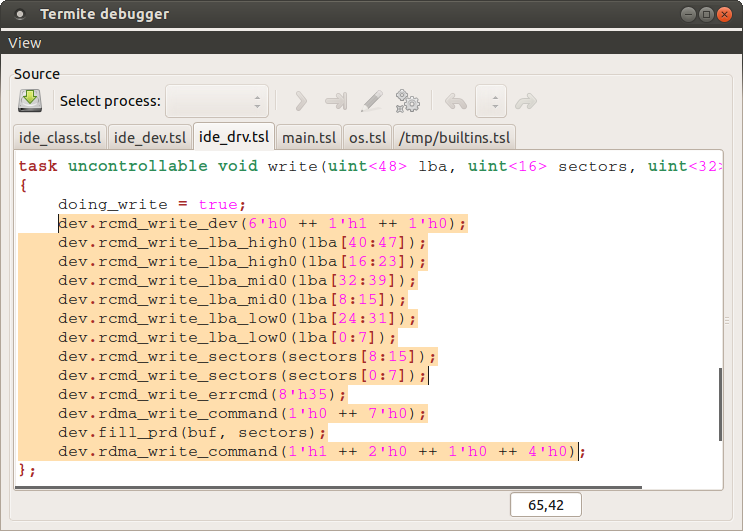
\includegraphics[width=\linewidth]{imgs/screenshot_write.png}
    \caption{Screenshot of \termite with a synthesised implementation of the IDE driver.  Automatically generated code is highlighted.}
    \label{f:screenshot_write}
\end{figure}

In our case studies, 60\% to 90\% of the code was generated fully automatically, with the rest of the code produced in a user-guided fashion. Drivers with complex interrupt handlers which had to be manually written tended to be near the 60\% end of the range. The others, which did not rely on interrupt handling such as the \iic driver (with synthesis walkthrough in Appendix~\ref{ch:worked_example}) were closer to the 90\% end of the range. Once an initial version of device and OS specifications was ready, it took us several hours to generate the driver implementation for each of our case studies.  Three quarters of this time was spent debugging the input specifications, with the rest of it spent generating driver source code with the help of the user-guided code generation GUI.

I found counterexample-driven debugging to be crucial to the productivity of synthesis-based development.  Before the debugger was available, I had to rely on code inspection to identify defects in the input specifications, which proved to be a frustrating and unpredictably long process.  The \termite debugger streamlines this process, giving us the confidence that any failure can be localised by following well-defined steps.  A typical debugging session takes a few minutes and involves entering only a few commands manually before the defect is localised. 

%We found the incremental approach to debugging and synthesis to 
%be the most effective.  Incremental synthesis 
%
%synthesise a single driver function or a small group of related 
%functions before adding m
%
%This is achieved by disabling invocations of all but one I/O 
%operations in the OS model. 
%
%Incremental synthesis

%In all case studies, we have been able to achieve human-readable 
%code structure that one would expect in a manually developed 
%driver.  60\% to 90\% of the code was generated fully 
%automatically and did not require any manual changes.  The rest of 
%the code was produced in a user-guided fashion, as described in 
%Section~\ref{s:user-guided}.  Human involvement was required for 
%three reasons.  First, it was necessary to get around the 
%white-box assumption, causing automatically generated code to 
%access variables outside the syntactic scope of the driver, as 
%explained in Section~\ref{s:user-guided}.  Second, it was used to 
%enforce a particular preferred implementation among several 
%functionally equivalent alternatives.  A common example of such a 
%situation, illustrated in Section~\ref{s:user-guided}, is 
%implementing I/O completions using interrupts instead of polling.  
%Finally, we relied on manual intervention to improve the structure 
%of synthesized code to make it compliant with the standard Linux 
%driver structure.

\subsection{Size of synthesised code} 
The last two columns of Table~\ref{t:size} compare the size of synthesised drivers to existing manually developed drivers.  Synthesised drivers are significantly more compact than conventional drivers for two main reasons.  First, as explained in Section~\ref{s:limitations}, we only synthesise the driver logic directly responsible for controlling the device.  Conventional drivers typically contain a large amount of boilerplate code managing various OS resources.  I believe that this code can and should be synthesised using complementary techniques.  At the moment this functionality is implemented manually as a wrapper around the synthesised driver. 

Second, conventional device drivers are often designed to support multiple similar devices with slightly different interfaces and capabilities.  This leads to code bloat, as the driver must implement multiple versions of various operations, as well as logic to dynamically discover device capabilities and choose the right implementation to use.  In contrast, every \termite driver supports one specific device model with a fixed set of features.  Drivers for similar devices can share common specification code, but are synthesised as separate source code modules.  This approach leads to simpler code and is preferable for platforms with a fixed set of peripheral devices, such as smartphones, where shipping drivers that support only the required devices enables smaller system image.
  
\subsection{Specification reuse}  
The Termite specification methodology ensures mutual independence of device and OS specifications, and thus facilitates their reuse.  I have not yet carried out a substantial evaluation of such reuse; however I report our limited experience based on synthesising two SPI drivers for the seL4 OS\@.  The corresponding OS specification was initially developed during the work on the SPI driver for the exynos chipset.  It was later used to synthesise a driver for the STM32F10 chipset.  I was able to reuse most of the original specification.  Minor changes (8 lines of code) were required in the part of the specification describing configuration functionality of the driver, since the STM SPI controller supports a number of ad hoc transfer modes.  I expect to observe similar pattern for other devices and operating systems: generic OS specifications can be reused with localised, device-specific changes required to support non-standard device features.

\subsection{Performance of synthesised drivers} 
Our synthesised drivers implement effectively identical device control logic to their conventional counterparts and therefore have similar performance.  I benchmarked the USB webcam driver, which is the most performance-critical one among the case studies.  I measured CPU load and data throughput generated by the conventional and synthesised drivers for varying bitrates.  I obtained identical results, modulo measurement errors, for both drivers in all cases.

